\section{Texture}
Le plaquage des textures est intimement lié à la géométrie en question. Le
moteur ne fait donc que très peu de travail comparé à la géométrie qui doit
projeter elle même la texture et donner, en fonction des informations de
collisions, la couleur au point demandé. 

\remark{Comme nous pouvons le voir dans le description de l'architecture,
la gestion des différents formats d'image n'est pas à la charge
de la géométrie.}

\subsection{Exemple}
La \tsl{fig. \ref{fig:texture}} présente un exemple de plaquage de texture
(ici, une grille en metal) sur une sphère.

\begin{figure}[h]
  \begin{center}
    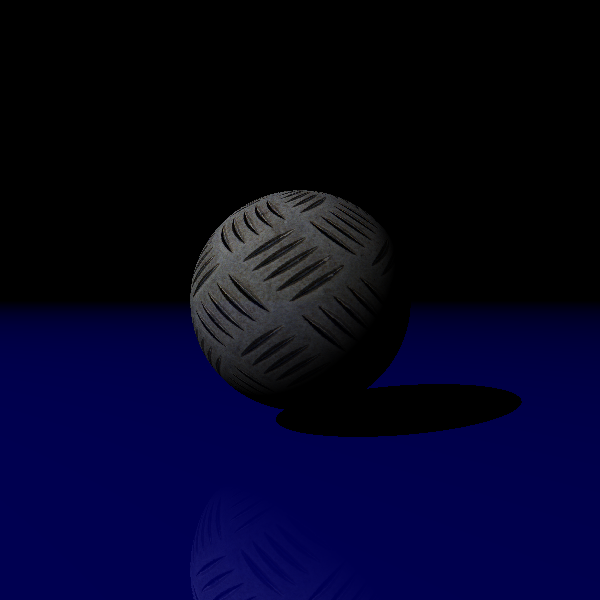
\includegraphics[width=.5\textwidth, keepaspectratio=true]{../../diary/17.png}
    \caption{Un exemple de rendu avec plaquage de texture\label{fig:texture} sur
    une sphère.}
  \end{center}
\end{figure}

\subsection{Amélioration \& bug connu}
Aucun.
